% Pursuing Stacks (cotes 134-2 to 134-8): archive cote 134-4, site page 55 (PDF page 56), typescript page 143.
% typescript. Draft compared: ps3.tex:2788-2862.
% AI-transcribed by Claude Opus 5.5 (claude-opus-5-5, adaptive thinking, effort high), Message Batches API, batch ps2 (msgbatch_01NVwr1Yuo8qJf5rykeGBXPK), 2026-11-12; image review recorded in records/CHECK_DECISIONS_134_3_4.tsv.
\scanpage{134-4/55}
\mspage{143}

d) of the proposition of page 121, in the present context, which we may
state in a more complete form as follows:

\uline{Proposition} Let M be a totally \xout{a\unsure{s|x}p} 0-connected category, W a geometric
saturated set of arrows in M . Assume moreover that for any two objects
in M, the object \uline{Hom}(X,Y) in M exists. Let X be an object of M, then
the following conditions \inserted{a) to c'')} are equivalent:
% Hand-drawn arrows are marked blue; typed objects remain plain.
\margin{\diagram{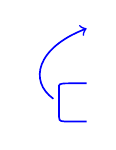
\begin{tikzpicture}[baseline=0ex,x=1em,y=1ex]\draw[color=blue,line width=.6pt] (1,-4.2)--(.2,-4.2)..controls(0,-4.2)and(0,-4)..(0,-3.8)--(0,-1.2)..controls(0,-1)and(.2,-1)..(.4,-1)--(1,-1);\draw[->,color=blue,line width=.6pt] (-.2,-2.3)..controls(-1.1,-.8)and(-.8,2)..(1,3.6);\end{tikzpicture}}}
\over{a)}{a'')} For any object Y, \uline{Hom}(Y,X) is W-aspheric over e \inserted{(i.e. it's map to e is ``universally in W'')}
\over{a')}{a''')} For any object Y, \uline{Hom}(Y,X) is $h_W$-contractible.
\over{\unsure{a'')}}{a)} For any object Y, \uline{Hom}(Y,X) is 0-connected.
\inserted{a') For any object Y, \uline{Hom}(Y,X) is W-aspheric (i.e. it's map to e is $\in W$).}
b)b')b'')\hand{b''')} same as above, with Y replaced by X.

\margin{\diagram{
\begin{tikzpicture}[baseline=0ex,x=1em,y=1ex]\draw[color=blue,line width=.45pt] (.15,1.5)..controls(-.1,0)and(-.1,-3)..(.15,-4.7);\end{tikzpicture}}}
c) For any object Y, $Y\hand{\rightarrow}$ \uline{Hom}(X,Y) is in W .
c') For any object Y, $Y\hand{\rightarrow}$ \uline{Hom}(X,Y) is W-aspheric\inserted{, i.e. is ``universally in W''.}
c'') For any object Y, Y as a subobject of \uline{Hom}(X,Y) is a deformation
ret\unsure{\over[typed]{ra}{ra}}ct with respect to $h_W$ .
\inserted{If moreover X has a section, these conditions are equivalent to:}
d) X is $h_{\hand{M}}$ - contractible.
d') X is $h_{\hand{W}}$-contractible.

\uline{Example} Let M=(Cat), the assumptions \inserted[typed]{on M} are clearly satisfied. If we take
for W the usual weak equivalences, it is clear too that W \xout{is} satisfies
a') and b) above i.e. \unsure{\over{W}{W}} is geometric. Thus the preceding proposition is
just an elaboration of the result stated after the prop. of page 97 -
which was the moment when it became clear that contractibility was an im-%
portant notion in the context of test categories and test functors, \xout{and}
which was the \inserted[typed]{main} motivation too for the \inserted[typed]{somewhat} lengthy trip through generalities on
homotopy notions,which is coming now (in the long last !) to a provisional
end...

To che\unsure{\over[typed]{c}{d}}k if the notions developped in this section are handy indeed,
I would still like to try them out in the case M is an elementary modelize\unsure{r}
A\^{} , corresponding to a test category A. But it's getting late this
night ...

\margin{55}
